\documentclass[11pt]{article}
\usepackage[utf8]{inputenc} % Para caracteres en espa�ol
\usepackage{amsmath,amsthm,amsfonts,amssymb,amscd}
\usepackage{multirow,booktabs}
\usepackage[table]{xcolor}
\usepackage{fullpage}
\usepackage{lastpage}
\usepackage{enumitem}
\usepackage{multicol}
\usepackage{fancyhdr}
\usepackage{mathrsfs}
\usepackage{wrapfig}
\usepackage[final]{pdfpages}
\usepackage{setspace}
\usepackage{esvect}
\usepackage{calc}
\usepackage{multicol}
\usepackage{cancel}
\usepackage{graphicx}
\graphicspath{ {picturesC/} }
\usepackage[retainorgcmds]{IEEEtrantools}
\usepackage[margin=3cm]{geometry}
\usepackage{amsmath}
\newlength{\tabcont}
\setlength{\parindent}{0.0in}
\setlength{\parskip}{0.05in}
\usepackage{empheq}
\usepackage{framed}
%\usepackage{newtxmath}
\usepackage{euscript}
\DeclareMathAlphabet{\mathpzc}{T1}{pzc}{m}{it}
\usepackage[most]{tcolorbox}
\usepackage{xcolor}
\colorlet{shadecolor}{orange!15}
\parindent 0in
\parskip 12pt
\geometry{margin=1in, headsep=0.25in}
\theoremstyle{definition}
\newtheorem{defn}{Definition}
\newtheorem{reg}{Rule}
\newtheorem{exer}{Exercise}
\newtheorem{note}{Note}
\newcommand{\volume}{{\ooalign{\hfil$V$\hfil\cr\kern0.08em--\hfil\cr}}}
\newcommand{\parr}{\mathbin{\|}} % Parralel Symbol
\begin{document}
\setcounter{section}{1}
\setcounter{page}{37}
\setcounter{equation}{71}
\def\thepart{\arabic{part}}
\setcounter{part}{7}
\numberwithin{equation}{part}

 \pagestyle{fancy}
\fancyhf{}
\rhead{Section 7:  Electrothermal Propulsion}
\rfoot{Page \thepage}
\thispagestyle{empty}

\begin{center}
{\LARGE \bf Section 7:  Electrothermal Propulsion}\\
{\large AE435}\\
Spring 2018
\end{center}
\vspace{5mm}
\section{Arcjets}
\vspace{25mm}
\tableofcontents
\newpage
\subsection{Discharge Physics}
Figure 6-12 in Jahn shows the electrical characteristic for a gaseous discharge.  Starting at the lowest discharge current and heading upwards: \newline \newline
\noindent\makebox[\textwidth]{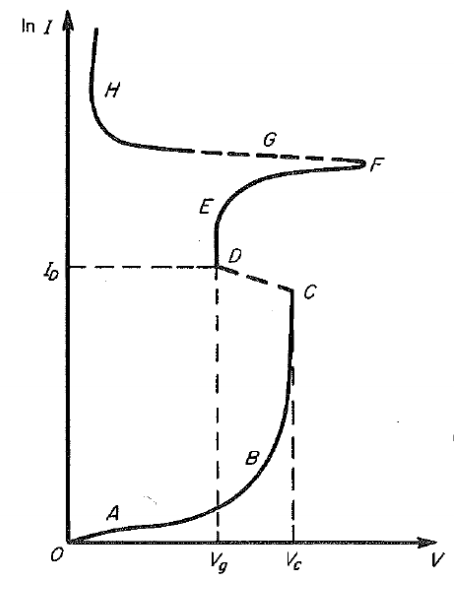
\includegraphics[scale=.97]{1.png}}
\newpage
 \begin{enumerate}
\item \textbf{O-A:} The \underline{\textbf{Stray Charge Region}}, here, ionization of gas is by background radiation, electrodes simply pick up bits of stray charge. There is very little ionization in this region. All the charged particles that we are collecting are due to stray ionization.
\item \textbf{A-B:}  The \underline{\textbf{First Townsend Region}}, where stray electrons pick up enough kinetic energy between collisions to ionize gas.  The current, $J \propto $ External Radiation Source Intensity, and so this is where Geiger-Muller counters operate. The electron has ionization collision with background neutral. We have enough electric field in this gap that any electron that gets created, now they are getting accelerated by that gap and have enough energy to collide.
\item \textbf{B-C:}  The \underline{\textbf{Second Townsend Region}}, where ions pick up enough kinetic energy from the E-field to cause \textbf{secondary electron emission} from the cathode. In this gap, ions pick up enough kinetic energy, a secondary electron comes off that cathode. The electron now accelerated towards the anode in the opposite direction. As it goes along that path it will have ionization collisions and create more ions.
\begin{center}
 \vspace{20mm}
  \textbf{Figure 12:}
 \end{center}
\item \textbf{C-D:}  \underline{\textbf{Sparking and Discharge Region}}, electron avalanche, lots of ionization and secondary electron emission. A self sustaining process of "steady discharge". The sparking discharge region curve here depends on
\begin{itemize}
\item Power supply characteristics
\item Gas pressure
\item Electrode material - Determines the secondary electron emission
\item Electrode shape
\begin{itemize}
\item Sharp points and/or high pressure lead to a \textbf{corona discharge}.
\begin{center}
 \vspace{30mm}
  \textbf{Figure 13:}
   \vspace{2mm}
 \end{center}
\item Blunt electrons and/or low pressure lead to a \textbf{glow discharge}.
\begin{center}
 \vspace{30mm}
  \textbf{Figure 14:}
   \vspace{2mm}
 \end{center}
\end{itemize}
\item Electrode spacing
\end{itemize}
\hspace{-10mm}\noindent\makebox[\textwidth]{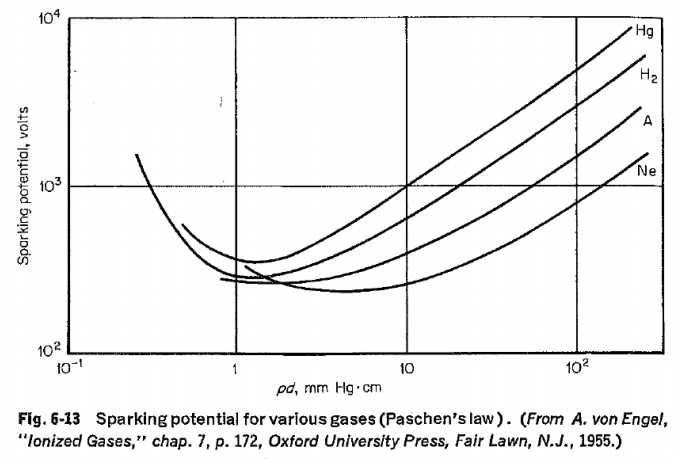
\includegraphics[scale=0.7]{2.png}}

From this figure, we have the relation between the gas pressure, electrode spacing and sparking potential. The voltage potential that is needed to get from region C to D. Figure 6-13 in Jahn shows "Paschen curve" of Vc as a function of   p d, where
\begin{itemize}
\item p is the pressure
\item d is the electrode gap
\end{itemize}
 \item \textbf{D-E:}  \underline{\textbf{Normal Glow Discharge Region}}, characterized by:
 \begin{itemize}
\item Constant current density ($10^{-3}$ to 1 $A/cm^2$)
\item High $T_e and low T_i\sim T_A$
\item Voltage drop primarily in cathode sheath
\end{itemize}
\item \textbf{E-F:}  \underline{\textbf{Abnormal Glow Discharge Region}}, where the
\begin{itemize}
\item Cathode drop starts to increase with current
\item Cathode heating grows proportionally
\end{itemize}
\newpage
\item \textbf{F-G:}  \underline{\textbf{Glow-to-Arc Transition Region}}, where the cathode temperature $T_c$ increase until thermionic emission starts to predominate.  Now, the cathode is really giving off electrons. Not only do we have secondary electron emissions but now since the cathode is so hot, electrons are popping off the surface because it so hot. "Thermionic Emission", meaning temperature driven emission. Also, field emission helps this process as well. If we have the cathode, there is also a plasma sheath that forms around the cathode. There will be a large potential drop that is relatively thin where the voltage drops orders of magnitude. As a result we have really strong electric fields right there at the surface. So we have a really strong field and the high temperature wanting to push electrons off the surface. The governing equation for this is:
 
 \begin{shaded}
 \textbf{Richardson-Duschman Relation}
 \begin{equation}
\begin{aligned}
j_e = A_r \, T_c^2 \, \exp \Bigg[\frac{-\Phi_{eff}}{k \, T_c}\Bigg]
\end{aligned}
\end{equation}
Where
 \begin{equation}
\begin{aligned}
A_r = 60\quad \Bigg[\frac{A}{cm^2 \, K^2}\Bigg]
\end{aligned}
\end{equation}
 \end{shaded}
 
and...
 
  \begin{shaded}
 \textbf{Effective Work Function}
 \begin{equation}
\begin{aligned}
\Phi_{eff} = \Phi_{w} - \sqrt{\frac{q_e \, E_c}{4 \, \pi \, \varepsilon_o}}
\end{aligned}
\end{equation}
Where
 \begin{equation*}
\begin{aligned}
\Phi_w&= \text{Zero-Field Work Function} \\
 E_c &= \text{Electric-Field Magnitude at the Cathode Surface} \\
\end{aligned}
\end{equation*}
 \end{shaded}
 Equation 7.74, the field reduces the work function required to push electrons off the surface. $\Phi_{eff}$ decreases the larger that electric field is. It is easier to pop the electrons off the surface. 
\newpage
Lowering the work function increase the emission current density. \\ \\
 \hspace{-20mm} \noindent\makebox[\textwidth]{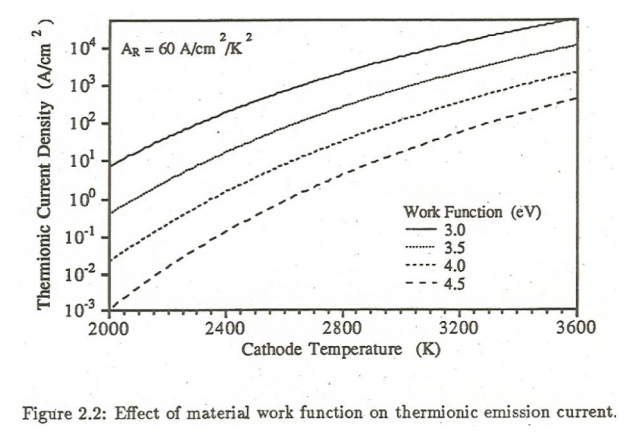
\includegraphics[scale=0.7]{3.png}} \\
Typical work functions for metal surfaces:

 \[ \scalebox{1.2}{
\begin{center}
 \begin{tabular}{c  c} 
Metal & $\Phi_w$ (V) \\[1ex] 
 \hline \hline
Si & 4.90 \\ 
Ni & 4.50\\ 
Mo & 4.30\\
W & 4.54\\[1ex] 
 \hline
\end{tabular}
\end{center}
 } \]
 
Mo and W are typically used in EP systems and often used for cathode materials.
 
Increased electric field has the same effect as lower work function: \\

\hspace{-10mm}\noindent\makebox[\textwidth]{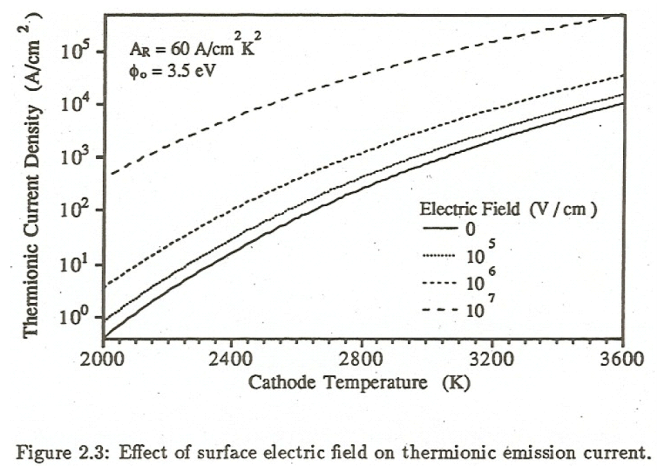
\includegraphics[scale=0.7]{5.png}}
 
Once thermionic emission sets in, the cathode drop decreases and the current increases.  The cathode temperature (and, thus, the emission current density) is regulated by the energy balance:
\begin{itemize}
\item Heating:  Ion bombardment and radiation
\item Cooling:  Conduction (to gas and solids), radiation, convection and electron emission
\end{itemize}
 \newpage
\item \textbf{G-H:}  \underline{\textbf{Arc}}, with resistance dropping rapidly enough that prompt kA currents, can vaporize electrodes. Classic fix, place a ballast resistor in series with the circuit:

\hspace{-10mm}\noindent\makebox[\textwidth]{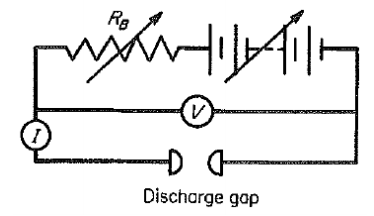
\includegraphics[scale=0.7]{6.png}}

\begin{equation*}
\begin{aligned}
V_B &= I \, R_B \\ \\
V_{tot} &= V_B + V_{gap} \\
\end{aligned}
\end{equation*}

As the current increases, the voltage drop across RB increases, preventing "runaway".

Note that G-H is the regime of interest for Electrothermal Thrusters Arcjet propulsion.
\end{enumerate}
In this figure, we have the set up for an arc jet. We have a voltage applied across some discharge gap, between the two electrodes. We have some low pressure region between that discharge gap. 
\newpage
\subsection{Arc Physics}
As we noted previously, an arc is struck when thermionic
emission causes runaway current. Figure 6-15 in Jahn
shows a schematic structures of an arc potential profile:

\hspace{-10mm}\noindent\makebox[\textwidth]{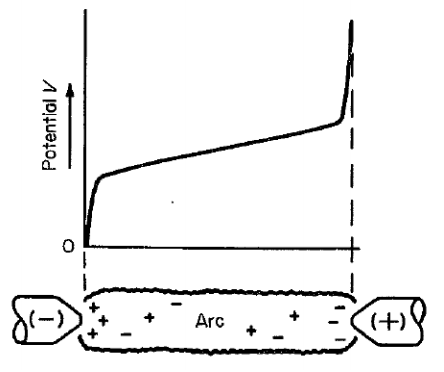
\includegraphics[scale=0.7]{7.png}}\\

Features:
\begin{enumerate}
\item \textbf{Cathode Sheath}, usually %only place where ions would really be moving....
\begin{enumerate}
\item A few Debye lengths $\lambda_D$ thick
\item A cathode fall, $V_c \sim \varepsilon_i$ , cathode fall on the order of
the ionization potential, this is the only region with
significant ion current; ions pick up enough energy
in the cathode fall to keep the cathode hot and
emitting.
\end{enumerate}
\item \textbf{Arc Column}, usually
\begin{enumerate}
\item Quasineutral, with ionization fraction 10-100% %Quasinuetrality only exist in the bulk. Bialtated at the sheath regions.
\item Near Complete Thermodynamic equilibrium, CTE, Te $\sim$ Tn
\item Electron current dominates here (no ion current)
\end{enumerate}
\item \textbf{Anode Sheath}, usually
\begin{enumerate}
\item A few Debye lengths $\lambda_D$ thick
\item Anode Fall, $V_a$
\begin{enumerate}
\item Electron-accelerating sheath,
\item Electron-repelling sheath, where column is more positive than anode.
\end{enumerate}
\end{enumerate}
\newpage
$ $

\begin{center}
 \vspace{60mm}
  \textbf{Figure 15:}
   \vspace{2mm}
 \end{center}
 
\textbf{Question: }Why would arc column have higher potential than the anode,  (Common in a lot of DC plasmas)?

\textbf{Answer: }Electrons are a mobile species, they will leave the plasma and leave behind a little bit of extra ion charge. This will cause the ions in the sheath to form like this. "It is Ion Repelling"
\end{enumerate}

\textbf{Magnetic Arc Constriction} - strong currents cause the arc to constrict, a "pinching" effect  which gives rise to instabilities

To illustrate, consider a cylindrical arc column, with:
\begin{itemize}
\item Radius $r_1$
\item Uniform current density
\end{itemize}
\begin{center}
 \vspace{70mm}
  \textbf{Figure 16:}
   \vspace{2mm}
 \end{center}

Ampere's law (2.96) for steady currents is:
\begin{equation}
\begin{aligned}
\nabla \times \vv{B} = \mu \, \vv{j}
\end{aligned}
\end{equation}

Taking the surface integral on a closed loop around the
column,

\begin{equation*}
\begin{aligned}
\int_S (\nabla \times \vv{B}) \cdot \mathrm{d}A = \int_S (\mu \, \vv{j}) \cdot \mathrm{d}\vv{A}
\end{aligned}
\end{equation*}

which by Stokes's theorem (2.73) is

\begin{equation*}
\begin{aligned}
\oint_c \vv{B} \cdot \mathrm{d}\vv{l} = \mu \int_S \vv{j} \cdot \mathrm{d}\vv{A}
\end{aligned}
\end{equation*}

Forcing the closed loop to be a circle of radius r, this
becomes

\begin{equation*}
\begin{aligned}
2 \, \pi \, r \, B_{\theta} = \mu \, \pi \, r^2 \, j \big|_{0}^{r_1}
\end{aligned}
\end{equation*}

So the azimuthal magnetic field strength is: 

\begin{equation}
\begin{aligned}
B_{\theta} = \left\{\begin{matrix}
\frac{\mu \, j \, r}{2} & \quad & 0 < r \leq r_1 \\ \\
\frac{\mu \, j \, r_1^2}{2 \, r} & \quad & r \geq r_1
\end{matrix}\right.
\end{aligned}
\end{equation}

The Mangetic field profile inside and outside of the arc. We have found the magnetic field but we still don't know why it pinches. The pinching is caused by a force. We are going to have a Lorentz force

This is shown in figure below (Jahn 6-16a).

\noindent\makebox[\textwidth]{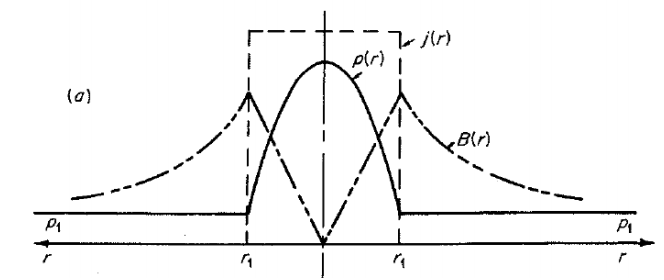
\includegraphics[scale=0.7]{8.png}}\\


Now recall the Lorentz force (2.66) with no Efield, on a single charge is:

Looking at the sketch above, if J is in this direction, what direction is the magnetic field. 
In the direction we draw the loop. Therefore the force F is going to be radially inwards.

\begin{equation*}
\begin{aligned}
\vv{F}_q = q \, \vv{v} \times \vv{B}
\end{aligned}
\end{equation*}

So the Lorentz force on a volume element dV with a number density n of charges is:

\begin{equation*}
\begin{aligned}
n \, \vv{F}_q \, \mathrm{d}\volume = n \, q \, \vv{v} \times \vv{B} \, \mathrm{d}\volume
\end{aligned}
\end{equation*}

or by definition of current density (2.51),
\begin{equation*}
\begin{aligned}
\vv{j} = n \, q \, \vv{v}
\end{aligned}
\end{equation*}
we have:
\begin{equation}
\begin{aligned}
\vv{f} = \vv{j} \times \vv{B} \qquad \bigg[\frac{N}{m^3}\bigg]
\end{aligned}
\end{equation}%Force acting on due to 

where we use a lower-case f to denote force density
(force per unit volume). So for this arc,

\begin{equation}
\begin{aligned}
\vv{f} = - \frac{1}{2} \, \mu \, j^2 \, \vv{r} \qquad \text{ for } \, r \leq r_1 
\end{aligned}
\end{equation} 

For all the regions we care about. There is no force outside of r1 because there is no arc there, there is no current there.

In equilibrium, this (inward) Lorentz force density is
balanced by the (outward) radial pressure gradient:

\begin{equation}
\begin{aligned}
\frac{\mathrm{d}p}{\mathrm{d}r} = - \frac{1}{2} \, \mu \, j^2 \, \vv{r}
\end{aligned}
\end{equation}
Integrating from r = 0 to r:
\begin{equation}
\begin{aligned}
p(r) = p_1 + \frac{1}{4} \, \mu \, j^2 \, (r_1^2 - r^2)
\end{aligned}
\end{equation}

where $p_1$ is the ambient pressure (outside the arc). Thus
the maximum pressure is at the core, on the centerline,
\begin{equation}
\begin{aligned}
p(0) = p_1 + \frac{1}{4} \, \mu \, j^2 \, r_1^2
\end{aligned}
\end{equation}
\newpage
The above analysis assumes UNIFORM current density.

Here's why this is unlikely:
\begin{enumerate}
\item The temperature distribution $T(r)$ is highest at the
center , $r = 0$
\item Since $p=nkT$ for a perfect gas, $n \sim$uniform through the
arc. Both $p$ and $T$ increase toward centerline such that
$n \sim$ constant
\item Since $j \perp B$ and $B \rightarrow 0$ at $r = 0$, the axial
conductivity also peaks at $r = 0$. No Bfield
on centerline to retard electron (current) motion.
\item End result: $\vv{j}$ is generally not uniform, as shown
in figure below.
\end{enumerate}


\hspace{-10mm}\noindent\makebox[\textwidth]{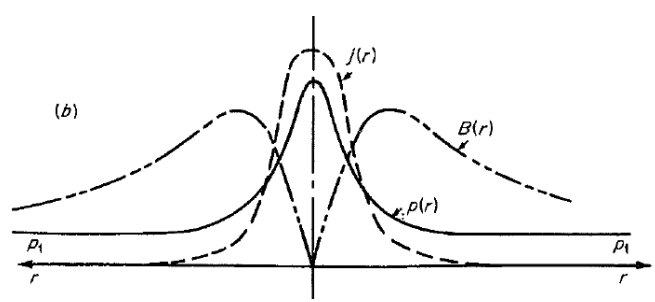
\includegraphics[scale=0.7]{9.png}}\\


Regardless of whether the current density is uniform or not uniform. 
\newpage 
This pinching process unfortunately leads to instability. For this process there are two types of instabilities:


\noindent\makebox[\textwidth]{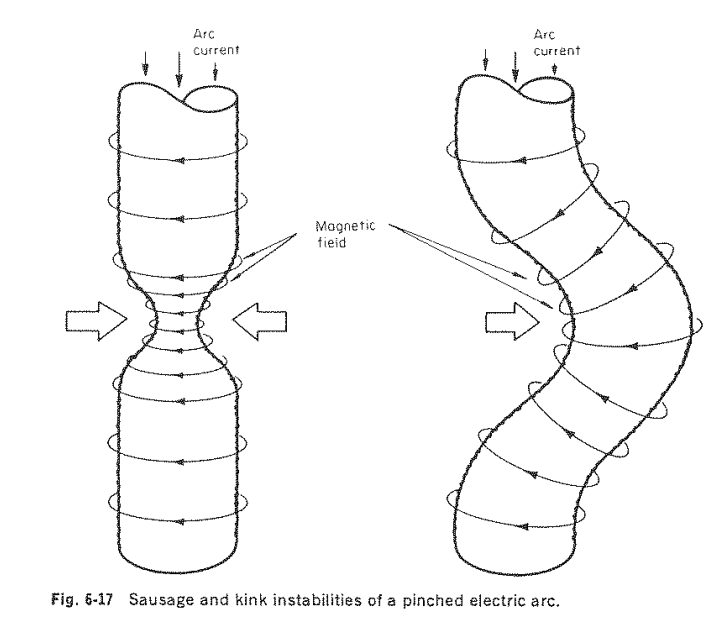
\includegraphics[scale=0.7]{10.png}}\\


\begin{enumerate}
\item \textbf{Sausage: } Since the arc current is:
\begin{equation*}
\begin{aligned}
J = \pi \, \int_0^{r_1} \, \vv{j}(r) \, r \, \mathrm{d}r \, \sim \, r_1^2
\end{aligned}
\end{equation*}
The force density in a constant current arc is
\begin{equation*}
\begin{aligned}
\vv{f} = - \frac{1}{2} \, \mu \, j^2 \, \vv{r} \, \sim \, - \frac{J}{r} \, \hat{r}
\end{aligned}
\end{equation*}
As a result, a small inward perturbation will grow, "necking" off the arc.
\item \textbf{Kink: }deflections of the arc tend to grow, since
forces are strong at smaller radii of curvature
\end{enumerate}
\textbf{Three Methods for Stabilizing an Arc: }
\begin{enumerate}
\item \underline{\textbf{Axial Magnetic Field: }}

Bfield confines arc to center, arc tunnels (for reentry - hypersonics studies) use this technique.
\item \underline{\textbf{Gas Vortex :}}

\hspace{-10mm}\noindent\makebox[\textwidth]{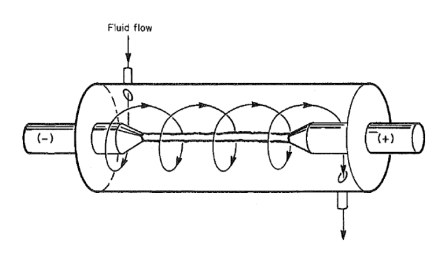
\includegraphics[scale=0.7]{11.png}}\\

In addition to stabilization, advantages include:
\begin{itemize}
\item Convection cools the walls
\item Longer fluid path increase the residence time, get
higher overall temperature
\item Injected gas cools the arc, lowering its conductivity
enabling higher operating voltage and higher power
\end{itemize}
\item \underline{\textbf{Constriction: }}

The pressure inside constriction will be high which keeps the arc from bending.

\hspace{-10mm}\noindent\makebox[\textwidth]{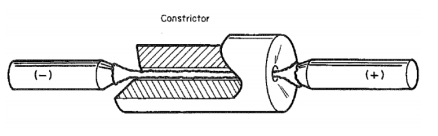
\includegraphics[scale=0.7]{12.png}}\\

\end{enumerate}
\newpage
\subsection{Modeling Approaches}
\subsubsection{Core Flow Model}
\hspace{-10mm}\noindent\makebox[\textwidth]{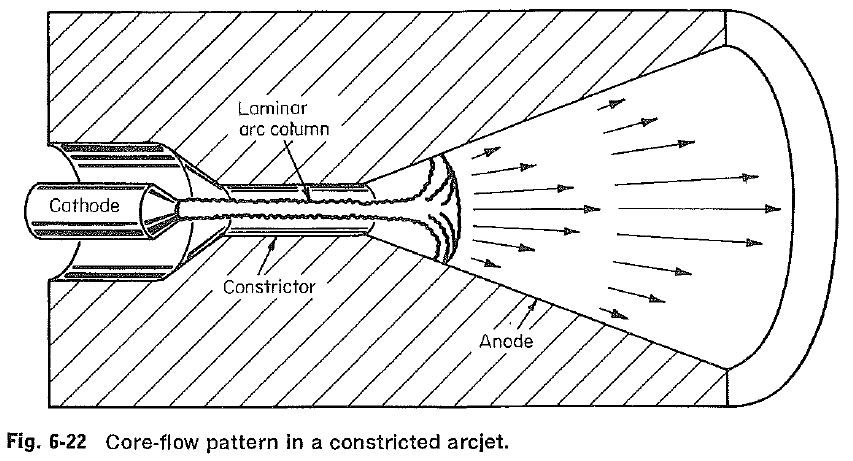
\includegraphics[scale=0.7]{1213.png}}\\
Assumptions:
\begin{itemize}
\item All heat input is in the arc column:
\begin{equation}
\begin{aligned}
P_{\text{in}} = \vv{j} \cdot \vv{E} = \sigma \, E^2
\end{aligned}
\end{equation}
Where
\begin{equation*}
\begin{aligned}
\sigma = \text{Electrical Conductivity}
\end{aligned}
\end{equation*}
\item Small diameter arc column with negligible gas flow
\item Cathode heated by cathode fall ($JV_c$), preheating gas
\item Constrictor heated by radiation from arc (optically thin gas)
\item Anode heated by anode fall ($JV_a$) upstream, convection downstream
\item Transparent column, LTE, no axial gradients
\end{itemize}

 \newpage
Thus the:
 \begin{shaded}
 \textbf{Energy Balance for a Core Flow Model Arc:}
 \begin{equation}
\begin{aligned}
\sigma \, E^2 = P_{\text{radiated}} - \frac{1}{r} \, \frac{\mathrm{d}}{\mathrm{d}r} \,\bigg(r \, k \, \frac{\mathrm{d}T}{\mathrm{d}r}\bigg)
\end{aligned}
\end{equation}
Where
\begin{equation*}
\begin{aligned}
P_r &= \text{Radiative Power Loss per Unit Volume} \\
k &= \text{Thermal Conductivity} \\
\end{aligned}
\end{equation*}
 \end{shaded}

These are tabulated for a variety of gases, at a given T, P.

The boundary conditions on the centerline are:
 
  \begin{equation*}
\begin{aligned}
\text{At} \, r = 0 \qquad T(0) = T_o \\ \\
\frac{\mathrm{d}T}{\mathrm{d}r} \bigg|_{r=0} = 0
\end{aligned}
\end{equation*}
 
Can then solve for core temperature $T_o(E)$.
 
For example, Jahn calculates for hydrogen at 1 atm with J = 150A:
\begin{center}
 \begin{tabular}{ c  c } 
 E  [V/cm]  & $T_o$  [K] \\ [1ex] 
 \hline
 25 & 20,000 \\ 
 100 & 40,000 \\
 250 & 60,000 \\[1ex] 
 \hline
\end{tabular}
\end{center}
for various voltage gradients (E) along the column.  These calculations also predict an arc diameter of 1-2mm.
 \newpage
\subsubsection{Heat Transfer:}

The same model can be used to calculate the heat transfer processes within the thruster block.  Expect the temperature profile to have a minima away from the walls:

\begin{center}
 \vspace{70mm}
  \textbf{Figure 17:}
   \vspace{2mm}
 \end{center}
 
Why:  The wall flow cools the walls, which soak up radiation from the arc.
 
Figure 6-23 shows thermal calculations (using core flow model) for a 30-kWe H2 arcjet.

\hspace{-10mm}\noindent\makebox[\textwidth]{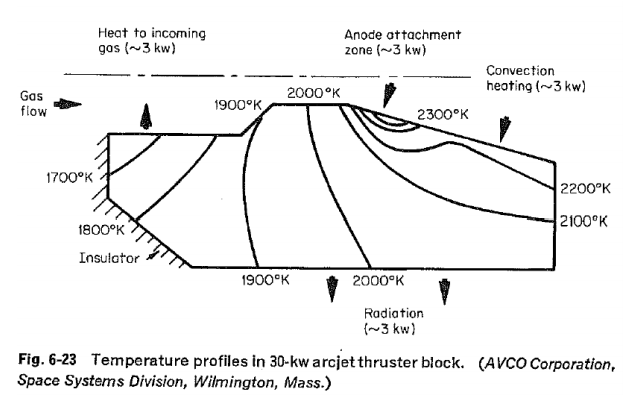
\includegraphics[scale=0.7]{13.png}}\\

Heat loss routes:
\begin{itemize}
\item 3kW to anode (by attachment and radiation)
\item 3kW to nozzle (by convection)
\item 3kW to the gas (by convection and conduction)
\item 3kW radiated to free space (gray body,     $\varepsilon \, \sigma \, T_{\text{external}}^4$             )
\end{itemize}

 
Figure 6-24 shows that there's significant regenerative cooling/heating, even with a solid anode.  In other words, there is significant heat transfer from the hot walls to the gas (like a resistojet).

\hspace{-10mm}\noindent\makebox[\textwidth]{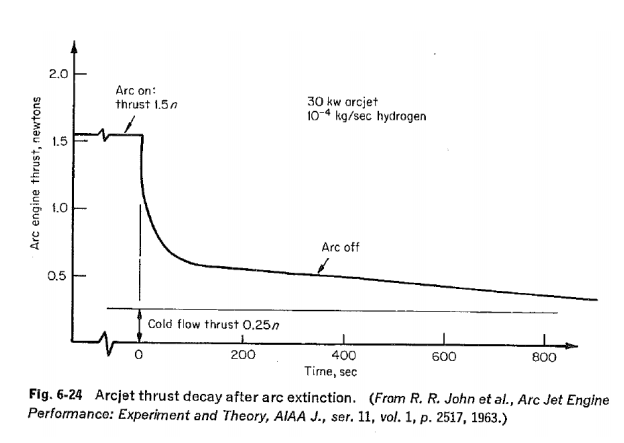
\includegraphics[scale=0.7]{14.png}}\\

The slow thrust decrease is due to heat transferred from the walls to the cool gas, even after the arc is shut off.
 \newpage
The core flow model neglects axial enthalpy flux to high-temperature gas in the arc column.  (7.83) was for radial energy flux only.  Clearly there is significant axial flux of high enthalpy gas.  The Stine-Watson model includes this:
   \begin{shaded}
 \textbf{Stine-Watson Model:}
 \begin{equation}
\begin{aligned}
\sigma \, E^2 = \rho \, u \, \frac{\mathrm{d}h}{\mathrm{d}z} - \frac{1}{r} \, \frac{\partial}{\partial r} \, \bigg(r \, k \, \frac{\mathrm{d}T}{\mathrm{d}r}\bigg)
\end{aligned}
\end{equation}

 \end{shaded}
 
Note this neglects radiative losses! Instead, we can use Stine-Watson model to solve for h(r,z). More sophisticated analyses take into account...

We need to solve for: Fluid dynamics in gas, Interface (sheath) models, Heat transfer to/from solid components

Meaning we need coupled equations for: Continuity, Momentum, Energy, Maxwell's Equations, Heat conduction in the solid, Constitutive relations ($\sigma(T)$, $k(T)$, $\mu(T)$)


  \begin{shaded}
 \textbf{General Equation for Arc Heating:}
 \begin{equation}
\begin{aligned}
\sigma \, E^2 = P_r - \frac{1}{r} \, \frac{\partial}{\partial r} \, \bigg(r \, k \, \frac{\mathrm{d}T}{\mathrm{d}r}\bigg) -\frac{\partial}{\partial z} \, \bigg(k \, \frac{\mathrm{d}T}{\mathrm{d}z}\bigg)+\rho \, u \, \frac{\mathrm{d}h}{\mathrm{d}z} +\rho \, v \, \frac{\mathrm{d}h}{\mathrm{d}r} - u \, \frac{\mathrm{d}p}{\mathrm{d}z} 
\end{aligned}
\end{equation}
Where
\begin{equation*}
\begin{aligned}
P_r &= \text{Radiated power} \\ \\
 \frac{\partial}{\partial r} \, \bigg(r \, k \, \frac{\mathrm{d}T}{\mathrm{d}r}\bigg)&= \text{Radial conduction} \\ \\
\frac{\partial}{\partial z} \, \bigg(k \, \frac{\mathrm{d}T}{\mathrm{d}z}\bigg) &= \text{Axial conduction} \\ \\
\rho \, v \, \frac{\mathrm{d}h}{\mathrm{d}r} &= \text{Radial convection} \\ \\
\rho \, u \, \frac{\mathrm{d}h}{\mathrm{d}z} &= \text{Axial convection} \\ \\
 u \, \frac{\mathrm{d}p}{\mathrm{d}z}  &= \text{Pressure work} \\
\end{aligned}
\end{equation*}
 \end{shaded}
To this energy equation must be added a momentum component. 
\begin{equation*}
\begin{aligned}
\rho \, u \, \frac{\mathrm{d}u}{\mathrm{d}z} + \rho \, v \, \frac{\mathrm{d}u}{\mathrm{d}r} = -  \frac{\partial p}{\partial z} + \frac{1}{r} \, \frac{\partial}{\partial r} \, \bigg(r \, \mu \, \frac{\mathrm{d}u}{\mathrm{d}r}\bigg)
\end{aligned}
\end{equation*}
Where the viscous force $\mu \, \frac{\mathrm{d}u}{\mathrm{d}r}$ will, in general, be important in the constrictor because of the small duct diameter. As such, the mass flux equation
\begin{equation*}
\begin{aligned}
2\pi\, \int_0^{r_c} \, \rho \, u \, r \, \mathrm{d}r = \text{constant}
\end{aligned}
\end{equation*}
is an appropriate equation of state for the boundary conditions on the arc axis and at the channel walls. 

By adding momentum and continuity to this and get something like the models shown in the handouts.  Real multiphysics model: rate chemistry, radiative losses, fluid dynamics
 
Megli, Krier, Burton - Thermophysics and Heat Transfer, Vol.10 No.4, 1996.
Axisymmetric, steady, laminar continuum flow, two-temperature, chemical non-equilibrium model for $N_2/H_2$ arcjet with gas swirl injection (includes azimuthal momentum eqn).

\hspace{-10mm}\noindent\makebox[\textwidth]{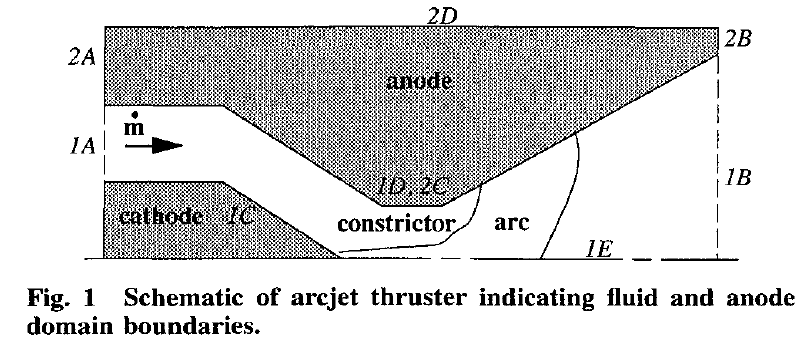
\includegraphics[scale=0.7]{15.png}}\\
\hspace{-10mm}\noindent\makebox[\textwidth]{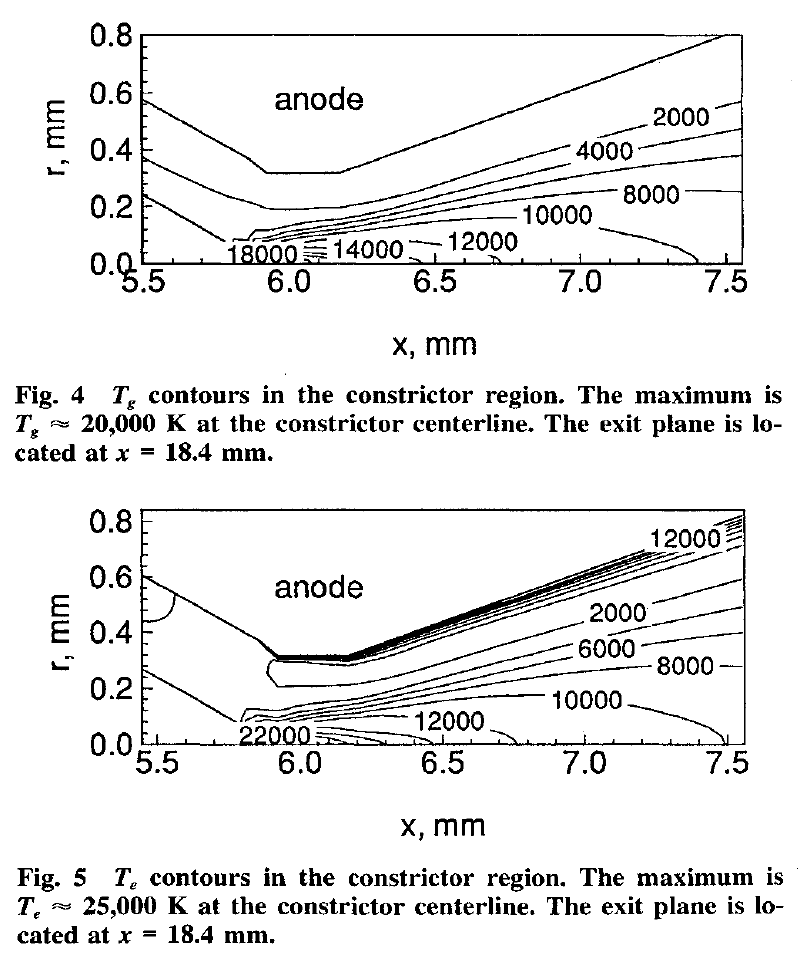
\includegraphics[scale=0.7]{16.png}}\\
\hspace{-10mm}\noindent\makebox[\textwidth]{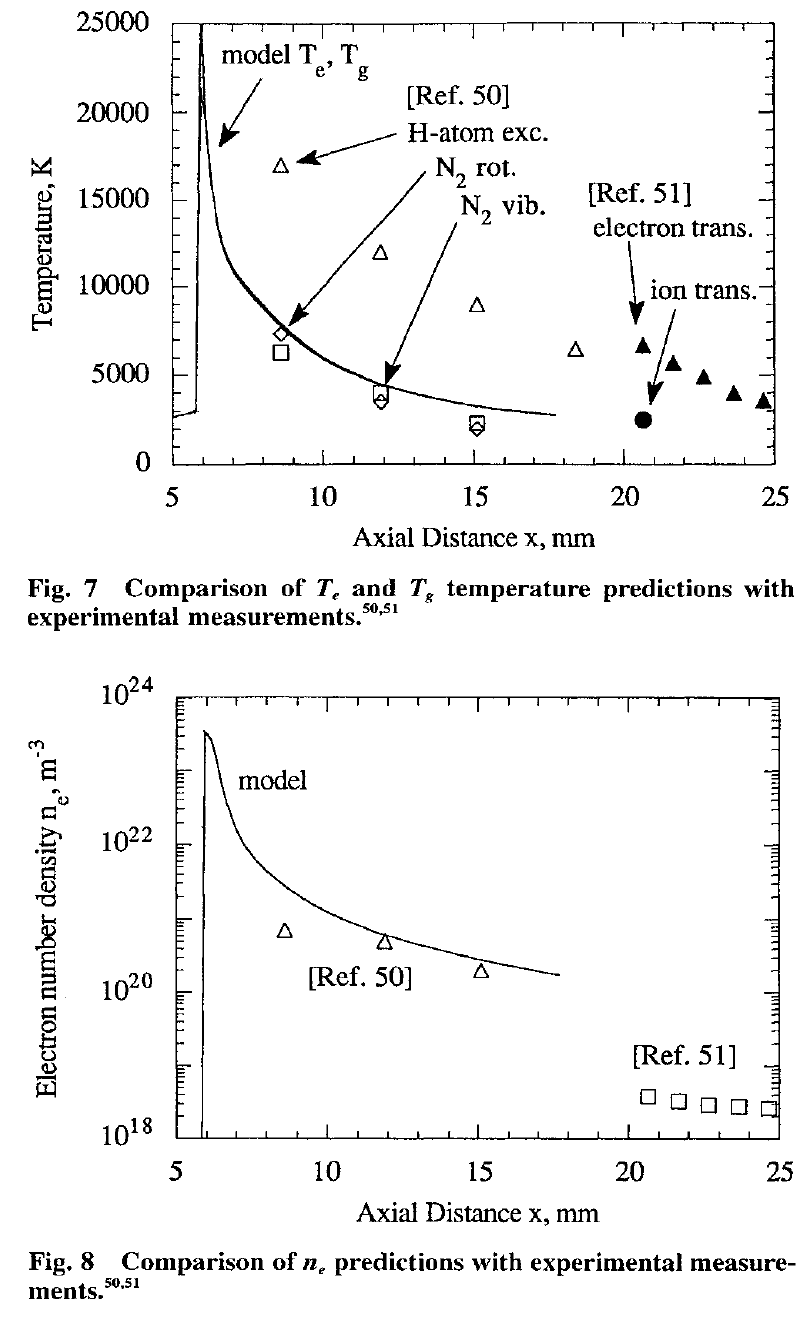
\includegraphics[scale=0.7]{17.png}}
\end{document}